Nous avons ensuite comparé l'évolution du temps d'intégration des opérations standards, \ie les opérations \emph{insert} et \emph{remove}, sur des documents LogootSplit et RenamableLogootSplit.
Puisque les deux types d'opérations partagent la même complexité en temps, nous avons seulement utilisé des opérations \emph{insert} dans nos benchmarks.
Nous faisons par contre la différence entre les mises à jours \emph{locales} et \emph{distantes}.
Conceptuellement, les modifications locales peuvent être décomposées comme présenté dans \cite{baquero2017pure} en les deux étapes suivantes :
\begin{enumerate}
  \item La génération de l'opération correspondante.
  \item L'application de l'opération correspondante sur l'état local.
\end{enumerate}
Cependant, pour des raisons de performances, nous avons fusionné ces deux étapes dans notre implémentation.
Nous distinguons donc les résultats des modifications \emph{locales} et des modifications \emph{distantes} dans nos benchmarks.
La \autoref{fig:evolution-integration-time-insert} présente les résultats obtenus.

\begin{figure}[!ht]
  \centering
  \subfloat[Modifications locales]{
      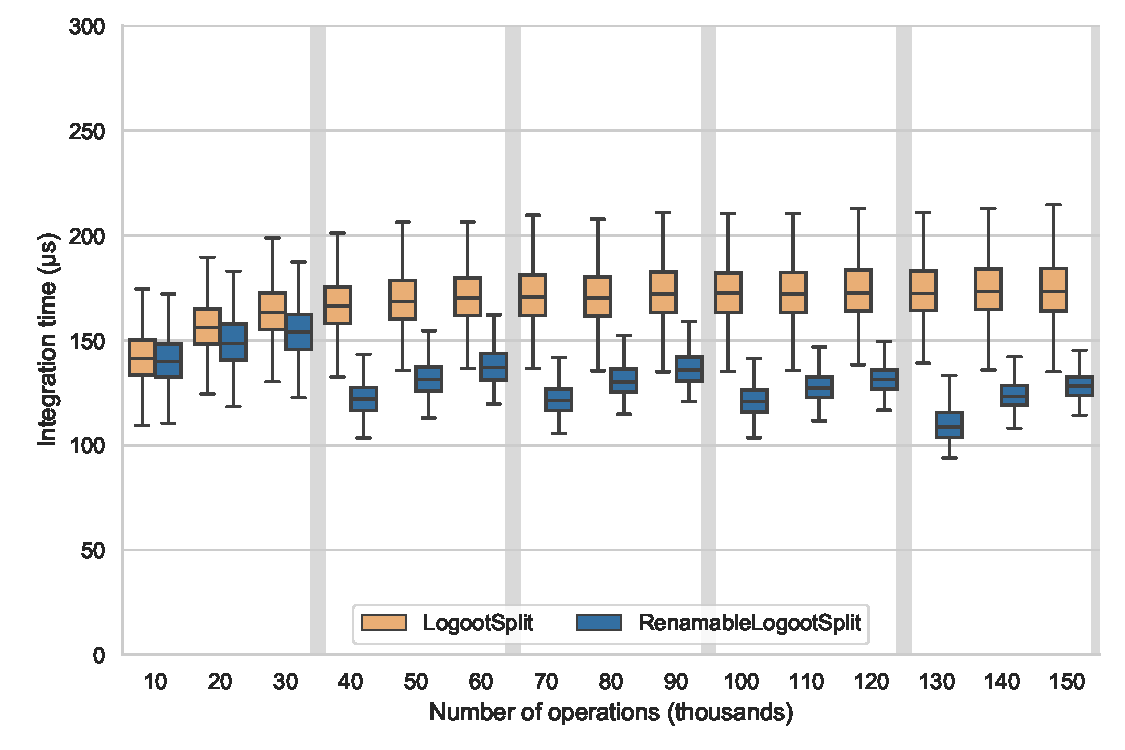
\includegraphics[width=0.45\columnwidth]{img/integration-time-boxplot-local-operations-without-outliers.pdf}
      \label{fig:evolution-integration-time-local-insert}}
  \hfil
  \subfloat[Modifications distantes]{
      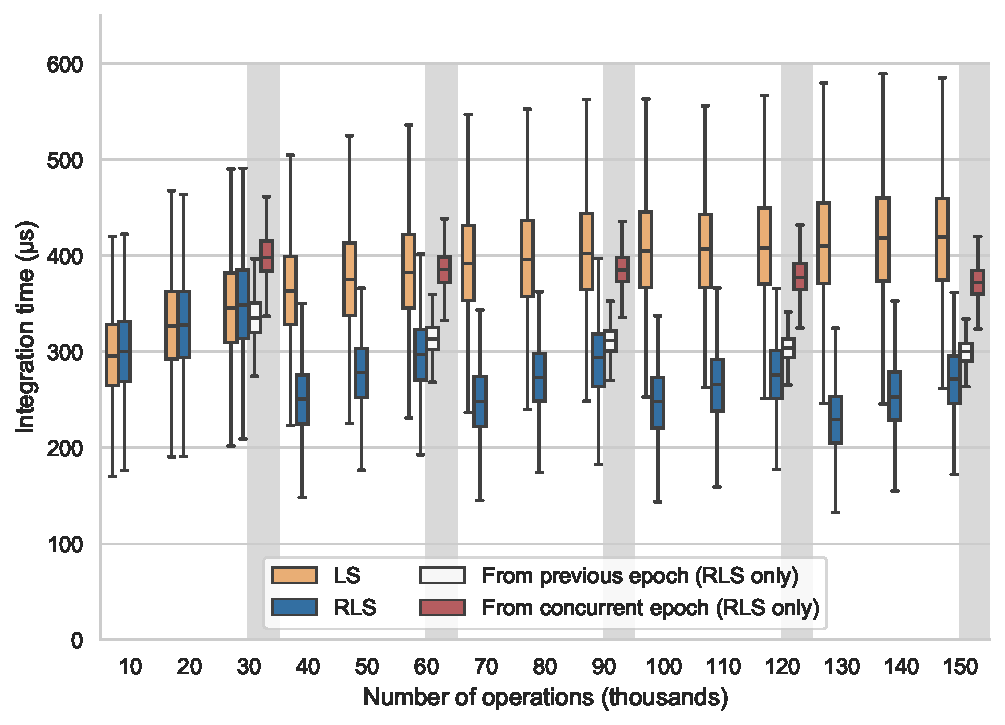
\includegraphics[width=0.45\columnwidth]{img/integration-time-boxplot-remote-operations-without-outliers.pdf}
      \label{fig:evolution-integration-time-remote-insert}}
  \caption{Temps d'intégration des opérations standards}
  \label{fig:evolution-integration-time-insert}
\end{figure}

Dans ces figures, les boxplots oranges correspondent aux temps d'intégration sur des documents LogootSplit, les boxplots bleues sur des documents RenamableLogootSplit.
Bien que les temps d'intégration soient initialement équivalents, les temps d'intégration sur des documents RenamableLogootSplit sont ensuite réduits par rapport à ceux de LogootSplit une fois que des opérations \emph{rename} ont été intégrées.
Cette amélioration s'explique par le fait que l'opération \emph{rename} optimise la représentation interne de la séquence (\ie elle réduit le nombre de blocs stockés dans l'arbre AVL).

Dans le cadre des opérations distantes, nous avons mesuré des temps d'intégration spécifiques à RenamableLogootSplit : le temps d'intégration d'opérations distantes provenant d'époques \emph{parentes} et d'époques \emph{soeurs}, respectivement affiché sous la forme de boxplots blanches et rouges dans la \autoref{fig:evolution-integration-time-remote-insert}.

Les opérations distantes provenant d'époques \emph{parentes} sont des opérations générées de manière concurrente à l'opération \emph{rename} mais appliquées après cette dernière.
Puisque l'opération doit être transformée au préalable en utilisant \textsc{renameId}, nous observons un surcoût computationnel par rapport aux autres opérations.
Mais ce surcoût est compensé par l'optimisation de la représentation interne de la séquence effectuée par l'opération \emph{rename}.

Concernant les opérations provenant d'époques \emph{soeurs}, nous observons de nouveau un surcoût puisque les noeuds doivent tout d'abord annuler les effets de l'opération \emph{rename} concurrente en utilisant \textsc{revertRenameId}.
À cause de cette étape supplémentaire, les performances de RenamableLogootSplit pour ces opérations sont comparables à celles de LogootSplit.

Pour récapituler, les fonctions de transformation ajoutent un surcoût aux temps d'intégration des opérations concurrentes aux opérations \emph{rename}.
Malgré ce surcoût, RenamableLogootSplit offre de meilleures performances que LogootSplit pour intégrer ces opérations grâce aux réductions de la taille de l'état effectuées par les opérations \emph{rename}.
Cependant, cette affirmation n'est vraie que tant que la distance entre l'époque de génération de l'opération et l'époque courante du noeud reste limitée, puisque les performances de RenamableLogootSplit dépendent linéairement de cette dernière (cf. \autoref{tab:time-complexity-operations}).
Néanmoins, ce surcoût ne concerne que les opérations concurrentes aux opérations \emph{rename}.
Il ne concerne pas la majorité des opérations, \ie les opérations générées entre deux séries d'opérations \emph{rename}.
Ces opérations, elles, ne souffrent d'aucun surcoût tout en bénéficiant des réductions de taille de l'état.
